\documentclass[12pt]{standalone}
\usepackage{graphicx,tikz}

\usetikzlibrary{arrows.meta}

\definecolor{uicred}{RGB}{228,78,97}
\definecolor{uicblue}{RGB}{0,179,230}
\definecolor{uicyellow}{RGB}{255,199,44}
\definecolor{uicdblue}{RGB}{20,95,170}

\usepackage{fontspec}
\setmainfont{Theinhardt Regular}

\begin{document}
\begin{tikzpicture}[arr/.style={-{Straight Barb[length=4pt,width=5pt]}}]
\fill[white,rounded corners=20pt] (-7.3,-3.5) rectangle (7.3,6.5);
\node (L) at (-4,0) {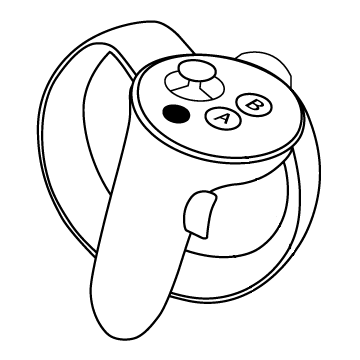
\includegraphics[width=5cm]{controlL.png}};
\node (R) at (3.95,0) {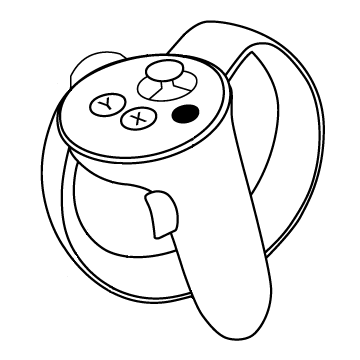
\includegraphics[width=5cm]{controlR.png}};
\node[uicred] (by) at (0,2) {Generate balls};
\node[uicyellow] (ax) at (0,.2) {Delete balls};
\node[uicblue] (grab) at (0,-.5) {Move balls};
\node[uicdblue] (joyR)[anchor=south] at (4,3) {\parbox{4cm}{\centering Click to toggle halos}};
\node[uicdblue] (joyRradius)[anchor=south] at (4,3.5) {\parbox{5cm}{\centering Move to change threshold}};
\node[uicdblue] (joyL)[anchor=south] at (-4,3) {\parbox{4cm}{\centering Click to toggle edges and triangles}};
\node[uicdblue,scale=2.5] at (0,5.5) {\bf Controls};
%% Connectors
\draw[uicred,line width=1pt,rounded corners=5pt] (by.west)--++(180:.5)--++(225:1.1);
\draw[uicred,line width=1pt,rounded corners=5pt] (by.east)--++(0:.5)--++(315:1.1);
\draw[uicyellow,line width=1pt,rounded corners=5pt] (ax.west)--++(180:1.55)--++(135:.63);;
\draw[uicyellow,line width=1pt,rounded corners=5pt] (ax.east)--++(0:1.55)--++(45:.63);;
\draw[uicblue,line width=1pt,rounded corners=3pt] (grab.west)--++(180:2.37);
\draw[uicblue,line width=1pt,rounded corners=3pt] (grab.east)--++(0:2.37);
\draw[uicdblue,line width=1pt,arr] (joyR.229)--++(270:1.15);
\draw[uicdblue,line width=1pt,arr] (joyL.295)--++(270:1.15);
\end{tikzpicture}
\end{document}